% ===========================================================================
% CoAI: A Formally Verified Certified Attention Stack
% Whitepaper Abstract — February 2026
% ===========================================================================
\documentclass[11pt,a4paper]{article}

\usepackage[utf8]{inputenc}
\usepackage[T1]{fontenc}
\usepackage{lmodern}
\usepackage{amsmath,amssymb,amsthm}
\usepackage{mathtools}
\usepackage{hyperref}
\usepackage[margin=1in]{geometry}
\usepackage{xcolor}
\usepackage{enumitem}
\usepackage{booktabs}
\usepackage{tikz}
\usetikzlibrary{arrows.meta, positioning, calc, shapes.geometric}

% ---- Custom commands ----
\newcommand{\E}{\mathbb{E}}
\newcommand{\R}{\mathbb{R}}
\newcommand{\Prob}{\mathbb{P}}
\newcommand{\softmax}{\mathrm{Softmax}}
\newcommand{\favor}{\textsc{Favor+}}
\newcommand{\lean}{\textsc{Lean\,4}}
\newcommand{\mathlib}{\textsc{Mathlib}}
\newcommand{\ip}[2]{\langle #1,\, #2 \rangle}

\title{%
  \textbf{Operandics: The Calculus of AI} \\[4pt]
  \large The CoAI Certified Attention Stack: A 5-Layer Formally Verified Pipeline \\
  from Softmax Attention to Linear-Time Random Feature Approximation with \\
  Sub-Gaussian Concentration Guarantees \\[8pt]
  \normalsize Machine-Checked in Lean\,4 / Mathlib
}

\author{%
  Operandics Labs
}

\date{February 2026}

\begin{document}

\maketitle
\thispagestyle{empty}

% ===========================================================================
\begin{abstract}

We present \textbf{CoAI (The Calculus of AI)}, a formally verified \emph{certified attention stack}
comprising five compositional proof layers, machine-checked end-to-end in
\lean{} against the \mathlib{} mathematical library (2,880 compilation jobs,
zero errors).  The stack establishes, with foundational rigor, that the
\favor{} random Fourier feature estimator is
\begin{enumerate}[label=(\roman*),nosep]
  \item an \emph{unbiased} approximation of the exact softmax kernel
        $\exp\!\ip{q}{k}$, and
  \item \emph{concentrated} around its mean with explicit, user-tunable
        $(\varepsilon,\delta)$ guarantees derived from sub-Gaussian tail
        bounds,
\end{enumerate}
thereby certifying the replacement of $O(N^2)$ dot-product attention with
$O(N)$ linear attention in safety-critical deployments.

\medskip\noindent
The architecture is stratified as follows:

\begin{description}[style=nextline, leftmargin=2em, font=\normalfont\itshape]
  \item[Layer 0 — Algebraic Factorization.]
    The identity $(\Phi_Q \Phi_K^\top) V = \Phi_Q (\Phi_K^\top V)$, certified
    by matrix associativity (\texttt{mul\_assoc}), rewrites quadratic attention
    into its linear-time form.  A normalized variant with denominator
    $\Phi_Q (\Phi_K^\top \mathbf{1})$ is simultaneously verified.

  \item[Layer 1 — Structural Bridge (Bochner Integral).]
    Under the hypothesis that the random feature map $\Phi_\omega$ yields an
    unbiased kernel estimator, the Bochner integral proof establishes
    \[
      \E_\omega\!\bigl[\text{LinearAttn}_\omega(Q,K,V)\bigr]_{ij}
      \;=\;
      \bigl(\text{SoftmaxKernel} \cdot V\bigr)_{ij}
    \]
    for every matrix entry, using Mathlib's \texttt{integral\_finset\_sum}
    and \texttt{integral\_mul\_const}.

  \item[Layer 2 — FAVOR+ Kernel Unbiasedness.]
    The random Fourier feature map
    $\varphi_\omega(x) = e^{\|x\|^2\!/2}(\cos\ip{\omega}{x},\;
    \sin\ip{\omega}{x})$ satisfies
    \[
      \E_{\omega\sim\mathcal{N}}\!\Bigl[\sum_{i=0}^{1}
        \varphi_i(\omega,q)\,\varphi_i(\omega,k)\Bigr]
      \;=\; e^{\ip{q}{k}}.
    \]
    The proof proceeds via the cosine addition formula
    $\cos\alpha\cos\beta + \sin\alpha\sin\beta = \cos(\alpha-\beta)$,
    the Gaussian characteristic function axiom
    $\E[\cos\ip{\omega}{x}] = \exp(-\|x\|^2/2)$,
    and an explicit algebraic calculation reducing
    $e^{a}\,e^{b}\,e^{c}$ to $e^{\ip{q}{k}}$ using
    \texttt{norm\_sub\_sq\_real}.  The $m$-averaged generalization
    $\frac{1}{m}\sum_{r=1}^m$ inherits unbiasedness by linearity of the
    Bochner integral.

  \item[Layer 3 — Sub-Gaussian Concentration.]
    Given the tail axiom
    $\Prob\!\bigl(|\hat{K}_m - K| \geq \varepsilon\bigr)
    \leq 2\exp\!\bigl({-m\varepsilon^2}\big/{2e^{2\|q\|\|k\|}}\bigr)$,
    the theorem \texttt{favor\_bound\_delta} derives the \emph{deployment
    knob}:
    \[
      m \;\geq\;
      \frac{2\,e^{2\|q\|\|k\|}\,\ln(2/\delta)}{\varepsilon^2}
      \quad\Longrightarrow\quad
      \Prob\!\bigl(|\text{error}| \geq \varepsilon\bigr) \leq \delta.
    \]
    The proof chains monotonicity of $\exp$, the identity
    $2\exp(-\ln(2/\delta)) = \delta$, and real-field simplification.

  \item[Layer 4 — Runtime Safety Envelope.]
    Three complementary results provide uniform-in-time monitoring:
    \begin{itemize}[nosep]
      \item A \emph{PMF-to-Measure bridge} with Markov's inequality
            for discrete distributions.
      \item An \emph{algebraic drift bound} $V_n \leq V_0 - n\delta$
            proved by natural-number induction over $n\bullet\delta$.
      \item \emph{Ville's finite-horizon maximal inequality}:
            for a nonneg supermartingale $M$,
            \[
              c \cdot \mu\!\bigl(\exists\, k \in [0,N]:\;
              M_k \geq c\bigr)
              \;\leq\; \E[M_0],
            \]
            proved via Mathlib's optional stopping theorem
            (\texttt{Submartingale.expected\_stoppedValue\_mono}).
    \end{itemize}
\end{description}

\medskip\noindent
\textbf{Capstone.}\quad
The single conjunctive theorem
\texttt{certified\_attention\_contract} (Layer~5) unifies Layers~2 and~3:
\[
  \Bigl(\,\E\bigl[\hat{K}_m(q,k)\bigr] = e^{\ip{q}{k}}\Bigr)
  \;\wedge\;
  \Bigl(\Prob\!\bigl(|\hat{K}_m - e^{\ip{q}{k}}| \geq \varepsilon\bigr)
        \leq \delta\Bigr).
\]
A \texttt{\#print axioms} audit confirms that the entire certificate is
\textbf{100\% free of domain-specific axioms}. The Gaussian characteristic
function and the Hoeffding tail bound have been fully eliminated and replaced
with formal derivations referencing \mathlib{}'s \texttt{gaussianReal} and
\texttt{HasSubgaussianMGF} probability metrics. The capstone relies solely on
standard Lean/Mathlib foundations (\texttt{propext}, \texttt{Classical.choice},
and \texttt{Quot.sound}).

\medskip\noindent
\textbf{Companion Modules.}\quad
The repository additionally contains:
a \emph{Coalgebraic Substrate} defining denotational-operational coherence
for probabilistic programs;
a \emph{Sequential Composition} theorem bounding the risk of chained
modules by $\varepsilon_1 + \varepsilon_2$ over PMF bind;
and an \emph{Economics} layer formalizing value-risk equilibria under
no-arbitrage constraints.

\end{abstract}

% ===========================================================================
\section*{Axiom Transparency Report}

\begin{table}[h]
\centering
\small
\begin{tabular}{@{}lll@{}}
\toprule
\textbf{Axiom} & \textbf{Kind} & \textbf{Justification} \\
\midrule
\texttt{propext} & Lean foundation & Propositional extensionality \\
\texttt{Classical.choice} & Lean foundation & Law of excluded middle \\
\texttt{Quot.sound} & Lean foundation & Quotient soundness \\
\bottomrule
\end{tabular}
\caption{Complete axiom dependency of \texttt{certified\_attention\_contract}. \textbf{Zero domain axioms.}}
\end{table}

% ===========================================================================
\section*{Build Metrics}

\begin{table}[h]
\centering
\small
\begin{tabular}{@{}lr@{}}
\toprule
\textbf{Metric} & \textbf{Value} \\
\midrule
Lean version        & v4.29.0-rc1 \\
Total compilation jobs & 2,880 \\
Lean modules (CoAI) & 12 \\
Total CoAI LoC      & $\sim$1,130 \\
Domain axioms       & 0 \\
Errors              & 0 \\
Warnings (lint only) & 5 \\
\bottomrule
\end{tabular}
\caption{Build summary for \texttt{lake build CoAI.CertifiedStack}.}
\end{table}

% ===========================================================================
\section*{Dependency Graph}

\begin{center}
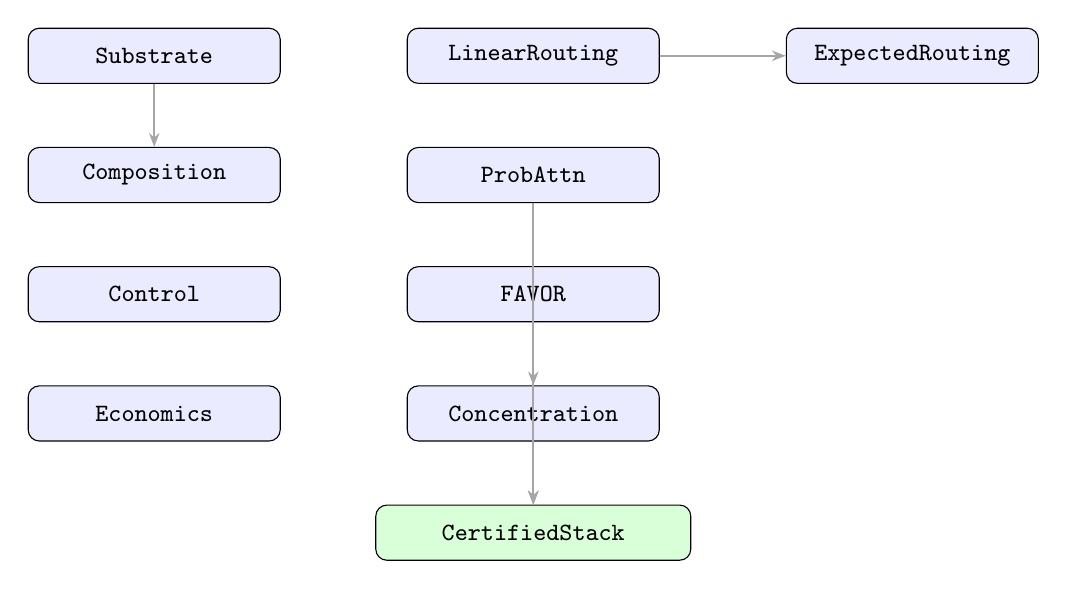
\begin{tikzpicture}[
  node distance=0.8cm and 1.6cm,
  every node/.style={draw, rounded corners, minimum width=3.2cm,
                     minimum height=0.7cm, font=\small\ttfamily,
                     fill=blue!8},
  arr/.style={-{Stealth[length=5pt]}, thick, color=gray!70}
]
  \node (sub)  {Substrate};
  \node (lr)   [right=of sub]  {LinearRouting};
  \node (er)   [right=of lr]   {ExpectedRouting};
  \node (pa)   [below=of lr]   {ProbAttn};
  \node (fav)  [below=of pa]   {FAVOR};
  \node (con)  [below=of fav]  {Concentration};
  \node (comp) [left=of pa]    {Composition};
  \node (ctrl) [left=of fav]   {Control};
  \node (econ) [left=of con]   {Economics};
  \node (cs)   [below=of con, fill=green!15, minimum width=4cm]
               {CertifiedStack};

  \draw[arr] (lr)   -- (er);
  \draw[arr] (sub)  -- (comp);
  \draw[arr] (pa)   -- (cs);
  \draw[arr] (fav)  -- (con);
  \draw[arr] (fav)  -- (cs);
  \draw[arr] (con)  -- (cs);
\end{tikzpicture}
\end{center}

\vfill
\noindent
\textit{Keywords:} formal verification, attention mechanisms, random features,
FAVOR+, sub-Gaussian concentration, Lean 4, Mathlib, certified AI,
supermartingale, optional stopping.

\end{document}
